% !TEX encoding = UTF-8 Unicode

\documentclass[a4paper]{article}

\usepackage{color}
\usepackage{xcolor}
\usepackage{url}
\usepackage[T2A]{fontenc} % enable Cyrillic fonts
\usepackage[utf8]{inputenc} % make weird characters work
\usepackage{graphicx}
\usepackage{amsthm}
\usepackage{amsmath}
\usepackage{booktabs,hhline}

\usepackage{multirow}       % used for making multirow tables (Nemanja)
\usepackage{minted}

%\usepackage[english,serbian]{babel}
\usepackage[english,serbianc]{babel} %ukljuciti babel sa ovim opcijama, umesto gornjim, ukoliko se koristi cirilica

\usepackage[unicode]{hyperref}
\hypersetup{colorlinks,citecolor=green,filecolor=green,linkcolor=blue,urlcolor=blue}

\newtheorem{primer}{Пример}[section] %ćirilični primer
%\newtheorem{primer}{Primer}[section]

\newtheorem{definic}{Дефиниција}
\newcommand{\norm}[1]{\left\lVert#1\right\rVert}

\begin{document}

%TODO smisliti naslov
\title{DeepDream\\ \large{Cањање и визуелизација конволутивних неуронских мрежа}\\ \small{Семинарски рад у оквиру курса\\\textit{Истраживање података}\\ Математички факултет}}

\author{Немања Мићовић\\ \texttt{nmicovic@outlook.com}}
\date{}
\maketitle

\abstract{
    Неуронске мреже у последњих неколико година добијају на значају услед ефикасне
    паралелизације њиховог тренинга што омогућава тренирање модела над великим
    скупом инстанци као и конструкцију архитектура које поседују велики број слојева.
    Иако постижу значајне резултате, интепретабилност и разумевање добијеног модела
    остаје отворен и нерешен проблем.

    Пројекат \texttt{DeepDream} за циљ има да визуализује објекте и шаблоне
    које је конволутивна мрежа научила. Добијена сликa се потом користи
    у генерисању нових слика у којима се амплификују појмови које је мрежа
    научила, како би се не крају добиле слике које многе подсећају на снове.
}


% ------------
% COVER IMAGE
% ------------
\begin{figure}[h!]
\begin{center}
    \includegraphics[width=\textwidth]{./resources/cover.jpg}
\end{center}
\end{figure}


\newpage
\tableofcontents

\newpage

% ---------------------------------------------------------------------------------------------------------------------
\section{Увод}
% ---------------------------------------------------------------------------------------------------------------------
Неуронске мреже постижу значајне резултате на многим пољима вештачке интелигенције.
Упркос томе, наше познавање њиховог интерног рада и интерпретабилност добијених модела, 
остају изненађујуће на ниском нивоу.

У делу \ref{sec:nn} дат је кратак преглед неуронских мрежа,
но услед сложености тематике, изложени материјал је више информативан него технички. За технички део
се препоручују књиге \cite{bishop, statisticalLearning, murphy}.

Део \ref{sec:deepdream} описује пројекат \texttt{DeepDream}.
Секција \ref{subsec:deepdreamGenerate} детаљније описује пројекат,
а \ref{subsec:generatingImages} приказује програмски код којим се неуронска мрежа
може натерати да \textit{сања}, односно омогућава генерисање слика које
поседују објекте које је мрежа научила да препознаје.

% ---------------------------------------------------------------------------------------------------------------------
\section{Неуронске мреже}
% ---------------------------------------------------------------------------------------------------------------------
\label{sec:nn}

% ---------------------------------------------------------------------------------------------------------------------
\subsection{Перцептрон}
% ---------------------------------------------------------------------------------------------------------------------
Перцептрон је први пример неурона који се појавио у области \cite{perceptronOriginal}. Оригинални перцептрон је
представљао бинарни класификатор који је могао да изврши класификацију уколико су инстанце линеарно сепарабилне,
а иначе тренинг не би успевао.

Класификација се врши формулом:

\[ f(x) =
  \begin{cases}
    1,      & \quad \text{ако } w \cdot x + b > 0\\
    0,      & \quad \text{иначе } \\
  \end{cases}
\]

Вектор реалних вредности означавамо са $w$ и називамо га \textit{тежине} (eng. \textit{weights}), вредност $b$ називамо пристрасност (eng. \textit{bias}),
a оператор $\cdot$ означава скаларни производ дефинисан као $\sum_{i=1}^m w_ix_i$.
Вредност $f(x) = 1$ означава да је инстанца $x$ класификована као \textit{позитивна}, a vrednost $f(x) = 0$ да је класификована
као \textit{негативна}.


Слика \ref{fig:perceptron} приказује перцептрон за $m=2$.

\begin{figure}[h!]
\begin{center}
    \includegraphics[scale=0.5]{./resources/perceptron.png}
\end{center}
\caption{Пецептрон}
\label{fig:perceptron}
\end{figure}

% ---------------------------------------------------------------------------------------------------------------------
\subsection{Неуронске мреже са пропагацијом унапред}
% ---------------------------------------------------------------------------------------------------------------------
Неуронска мрежа са пропагацијом унапред састоји се из више слојева који садрже \textit{неуроне}. Слојеви између улаза
и излаза се називају \textit{скривени слојеви} (eng. \textit{hidden layers}). Неурон представља
рачунску јединицу сличну перцептрону. Оно што је кључно у неуронским мрежама јесте нелинеарност која се уводи
код неурона, чиме се омогућава да неуронска мрежа изврши класификацију и нелинеарно сепарабилних инстанци.
Постоји и теорема која гарантује да неуронска мрежа са једним скривеним слојем може апроксимирати произвољну функцију.

Неуронске мреже могу имати више неурона на улазу и излазу и њихов број варира од архитектуре, скупа података и домена примене.
Често су улази у неуронску мрежу атрибути и представљају
делове улазних података (на пример број соба за одређивање цене куће).
На слици \ref{fig:nnet} приказана је неуронска мрежа са $n$ улаза и $m$ излаза.

Тренинг неуронске мреже се врши алгоритмом пропагације уназад (eng. \textit{backpropagation}). Више о алгоритму
и математичкој формулацији о неуронским мрежама може се пронаћи у \cite{bishop, statisticalLearning, murphy}.

\begin{figure}[h!]
\begin{center}
    \includegraphics[width=\textwidth]{./resources/neuralnet.png}
\end{center}
\caption{Неуронска мрежа са пропагацијом унапред}
\label{fig:nnet}
\end{figure}

% ---------------------------------------------------------------------------------------------------------------------
\subsection{Конволутивне неуронске мреже}
% ---------------------------------------------------------------------------------------------------------------------
Идеја о конволутивним неуронским мрежама јавила се још раних деведесетих \cite{covnetBirth},
но праву популарност конволутивне мреже достижу у последњих неколико година услед могућности
да се процес тренинга мрежа ефикасно паралелизује на графичким картицама. Успешна паралелизација
је омогућила да се врши тренинг над милијардама података као и да се користe дубоке неуронске мреже
са по неколико хиљада слојева. Популарност конволутивних мрежа нагло пораста, а сама тема постаје
изузетно истраживачки популарна.

Конволутивне неуронске мреже постигле су изузетне резултате у проблемима попут класификације \cite{krizhevsky,
ciregan, DBLP:journals/corr/SimonyanZ14a},
а генерално се могу користити када је у питању нека врста улазног сигнала (слика, звук, видео). Коришћене су и
за класификацију текста \cite{cnnForText} а занимљива је и примена у раду \cite{cnnForAutism}.

Конволутивне мреже се могу применити на било какве податке који поседују структуралну информацију.
Другачије речено, уколико се редослед података/сигнала једне инстанце пермутује, губи се суштина информације.
На пример, уколико се пермутују пиксели слике, губи се информација као и сам објекат који је на слици.

Неурони конволутивне мреже уче да препознају неку врсту шаблона на основу тренинг скупа. Што је неурон дубље у мрежи,
шаблон који препознаје постаје комплекснији. На примеру слике при препознавању лица,
један од неурона у почетним слојевима би препознавао хоризонталну линију, а неурон при крају, очи или нос. Комбинација неурона
омогућава да се дође до одговора шта је на слици. Често се на крају користи софтмакс техника (eng. \textit{softmax}) како би се
неурони на последњем слоју користили за оцену вероватноће класе којој инстанца припада \cite{bishop}.

Слика \ref{fig:cnn} приказује пример конволутивне мреже. У делу \ref{subsec:arch} ће детаљније бити образложени делови типичне архитектуре.

\begin{figure}[h!]
\begin{center}
\includegraphics[width=\textwidth]{resources/typical-cnn.png}
\end{center}
\caption{Пример архитектуре конволутивне неуронске мреже}
\label{fig:cnn}
\end{figure}

\subsubsection{Архитектура конволутивне мреже}
Архитектура конволутивне мреже се састоји из више слојева.
Слојеви су најчешће:
\begin{itemize}
    \item Потпуно повезани слој (eng. \textit{fully connected})
    \item Конволутивни слој (eng. \textit{convolutive})
    \item Слој агрегације (eng. \textit{pooling})
\end{itemize}

\paragraph{Потпуно повезани слојеви}
Потпуно повезани слој је сличан стандардним неуронским мрежама и често се користи на крају мреже заједно
са софтмакс функцијом како би се оцениле вероватноће класе.
Сликe \ref{fig:nn} и \ref{fig:cnn} приказују разлику између обичне неуронске мреже и конволутивне неуронске мреже,
слика \ref{fig:covnet} приказује пример архитектуре једне конволутивне мреже,
а слика \ref{fig:vgg16} приказује мрежу \texttt{VGG16} (eng. Visual Geometry Group) која је победила на такмичењу ILSVRC 2014
(видети део \ref{subsubsec:ilsvrc}).

\label{subsec:arch}

\begin{figure}[!tbp]
    \centering
    \begin{minipage}[b]{0.45\textwidth}
        \includegraphics[width=\textwidth]{resources/neural_net}
        \caption{Неуронска мрежа}
        \label{fig:nn}
    \end{minipage}
    \hfill
    \begin{minipage}[b]{0.45\textwidth}
        \includegraphics[width=\textwidth]{resources/cnn}
        \caption{Конволутивна неуронска мрежа}
        \label{fig:cnn}
    \end{minipage}
\end{figure}

\begin{figure}[h!]
\begin{center}
    \includegraphics[scale=0.2]{./resources/covnet2.png}
\end{center}
\caption{Пример архитектуре конволутивне мреже}
\label{fig:covnet}
\end{figure}


\begin{figure}[h!]
\begin{center}
    \includegraphics[width=\textwidth]{./resources/vgg16}
\end{center}
\caption{Мрежа VGG16}
\label{fig:vgg16}
\end{figure}

\paragraph{Конволутивни слојеви}
Конволутивни слој врши конструкцију нових атрибута који се потом
прослеђују даље у мрежу \cite{bishop, ni}. Често се на истом слоју дефинише више
паралелних конволутивних слојева. Паралелни конволутивни слојеви
могу на пример препознавати где су хоризонталне и вертикалне линије,
док ће се у наредним слојевима та информација користити да се препознају
комплекснији облици. Конволутивни слој \textit{превлачи} филтер преко
(на пример) слике и тиме детектује присуство одређеног атрибута на слици.
Овај процес се назива \textit{конволуција}.
Процесом тренинга атрибути које конволутивни слој тражи се уче. Величине
филтера су типично мале, на пример 2$\times$2 или 3$\times$3 пиксела на примеру слика.

Слика \ref{fig:filters} приказује филтере које је научила мрежа коришћена у раду \cite{krizhevsky}.

\begin{figure}[h!]
\begin{center}
    \includegraphics[width=\textwidth]{./resources/filters}
\end{center}
\caption{Пример филтера које је научила конволутивна мрежа}
\label{fig:filters}
\end{figure}

\begin{figure}[h!]
\begin{center}
    \includegraphics[scale=0.3]{./resources/maxpooling.png}
\end{center}
\caption{Агрегација која користи функцију максимума}
\label{fig:maxpooling}
\end{figure}

\paragraph{Слој агрегације}
Агрегациони слој израчунава функцију укрупњавања над улазом, најчешће
просек или максимум, и на тај начун укрупњава информације које добија
из претходног слоја \cite{ni}. Често слоју агрегације претходи конволутивни слој.
Уколико се улаз агрегира са 2$\times$2 филтером, онда је излаз агрегационог
слоја 2 пута мањи од свог улаза. На овај начин се смањује садржај али задржава
суштина.

Колико се заиста губи на информацији у агрегационом слоју? Уколико се користи
агрегациона функција за маскимум (слика \ref{fig:maxpooling}), онда се при укрупњивању губи информација
о томе где тачно налази атрибут који је детектован, али не и информација о томе
да ли је он детектован, што је најчешће сасвим довољно за проблем класификације.

Губитак на прецизности о позицији атрибута такође чини мрежу робуснијом
и омогућава већи степен генерализације \cite{bishop}. Тиме се допушта да позиција
атрибута на слици буде флексибилнија. На пример уколико се препознаје слово
А, врх слова (који личи на шпиц) ће се очекивати у средини слике и то на
горњој половини, али ће бити допуштено да позиција буде слободнија. Атрибут
(врх слова А) неће бити изгубљен при слоју агрегације који користи функцију за максимум.

\subsubsection{Визуелизација конволутивне мреже}
Велике конволутивне мреже су показале изузетне резултате у класификацији \cite{krizhevsky},
али до скоро није постојало дубоко разумевање зашто дају тако добре резултате или како
се могу побољшати. Рад \cite{visualizeCovnet} се бави њиховом визуелизацијом и један
од резултата јесте нова архитектура конволутивне мреже које је постигла боље резултате
од тадашњих (година 2014.) најбољих. Рад \cite{visualizeCovnet1} приказује како се конволутивне
неуронске мреже могу заварати користећи технику реактивације неурона са градијентним успоном.
Издвајање атрибута и њихово разумевање и интерпретација остају тежак проблем, чак и када су над визуелним подацима.
Неколико метода предложени су у радовима \cite{visualizeCovnet2, visualizeCovnet4, visualizeCovnet3}.

Пројекат \texttt{DeepDream} приказан у делу \ref{sec:deepdream} је делом мотивисан
потребом за дубљим разумевањем функционисања конволутивних мрежа.

\subsubsection{Такмичење ILSVRC}
\label{subsubsec:ilsvrc}
Најпознатији скуп података у области класификације слика је \textit{ImageNet} који се
користи на такмичењу \textit{ILSVRC}. \textit{ImageNet} за циљ има да понуди барем 1000 слика
за сваки скуп синонима у бази \textit{WordNet} којих има преко 100 000 инстанци.

Google је 2010. године организовао такмичење \textit{The ImageNet Large Scale Visual Recognition Challenge (ILSVRC)}
чија је тема била класификација и препознавање објеката на сликама. Такмичење је за циљ имало да мотивише истраживаче
да даље развијају алгоритме за класификацију објеката на сликама као и да им омогући да своје резултате
могу да упоредe са другима у области. Такмичење се оджава сваке године почевши од 2010. и представља један од
најбитнијих догађаја у овом делу области машинског учења.

Oко 2011. године, грешка класификације на такмичењу је била 25\%, 2012. године је дубока
неуронска мрежа постигла 16\%, а у следећих неколико година је грешка je драстично падала. Слика \ref{fig:imgneterror}
приказује грешку класификације на неколико узастопних такмичења. Занимљиво је поменути да су 2015. године и Microsoft
и Google успели да постигну мању грешку од човека (5.1\%), 4.94\% и 4.9\% респективно.

\begin{figure}[h!]
\begin{center}
    \includegraphics[width=\textwidth]{resources/ilsvrc.png}
\end{center}
\caption{Грешка класификације на скупу \textit{ImageNet}}
\label{fig:imgneterror}
\end{figure}



% ---------------------------------------------------------------------------------------------------------------------
\section{Deep dream}
\label{sec:deepdream}
% ---------------------------------------------------------------------------------------------------------------------
\texttt{DeepDream} представља пројекат који је конструисао Google. Главна мотивација за пројекат било је
интересовање истраживача да разумеју и визуализују како се понашају неурони утрениране конволутивне
мреже.

Реч сан (eng. \textit{dream}) се налази у називу јер је истраживаче ово
подсећало на визуелизацију снова. Google је на неки реч брендирао реч
\textit{сањати} (eng. \textit{dreaming}) у овом контексту и њена употреба је честа када
се мисли на процес генерисања слика које проузрокују тражене активације у тренираној мрежи.

Приступ који се користи је да се утренираној конволутивној неуронској мрежи којa препознаје слике
проследи нека произвољна слика, а онда се прослеђена слика мења тако да што више активира циљани
слој неуронске мреже. Део \ref{subsec:deepdreamGenerate} ће прецизније изложити процес генерисања слике.

\begin{figure}[h!]
\begin{center}
    \includegraphics[width=\textwidth]{./resources/deepdream1.jpg}
\end{center}
\caption{Пример слике пројекта \texttt{DeepDream}}
\label{fig:deepdream1}
\end{figure}

\begin{figure}[h!]
\begin{center}
    \includegraphics[width=\textwidth]{./resources/deepdream2.jpg}
\end{center}
\caption{Пример слике пројекта \texttt{DeepDream}}
\label{fig:deepdream2}
\end{figure}

\subsection{Генерисање слика}
\label{subsec:deepdreamGenerate}
Процес генерисања слике истраживачки тим је називао \textit{сањање} (eng. \textit{dreaming}),
и једна од инспирација су им били снови. Добијене слике поседују халуциногени ефекат који
многе подсећа на снове. Слике \ref{fig:deepdream1} и \ref{fig:deepdream2} приказују неке од добијених слика.

Једна од највећих замерки које постоје за неуронске мреже јесте неинтерпретабилност модела, те је од велика
важности да постоји барем неки начин да се објасни добијени модел.
Визуелизација мреже игра врло битну улогу јер омогућава да се провери шта је то мрежа научила. Уколико мрежа
учи да препознаје да ли је нешто банана или не, било би добро од мреже добити одређене слике о томе шта је за
мрежу банана, а шта није (слика \ref{fig:banana}). Слика \ref{fig:dumbbell} приказује шта за неуронску мрежу
значи тег. Може се приметити да је услед слика која су садржале људску руку која држи тег, мрежа научила
да је рука саставни део тега.

%\begin{figure}[h!]
%\begin{center}
    %\includegraphics[width=\textwidth]{./resources/noise-to-banana.png}
%\end{center}
%\caption{Пример визуелизације, Google}
%\label{fig:banana}
%\end{figure}

\begin{figure}[!tbp]
    \centering
    \begin{minipage}[b]{0.45\textwidth}
        \includegraphics[width=\textwidth]{./resources/noise-to-banana.png}
        \caption{Визуелизација мреже која препознаје банане}
        \label{fig:banana}
    \end{minipage}
    \hfill
    \begin{minipage}[b]{0.45\textwidth}
        \includegraphics[width=\textwidth]{./resources/dumbbells.png}
        \caption{Визуелизација мреже које препознаје тегове}
        \label{fig:dumbbell}
    \end{minipage}
\end{figure}

Техника коју Google користи је да се мрежи проследи одређена слика,
мрежа се пусти да изврши детекцију, а потом се бира слој и врши се
амплификација дела слике који је слој детектовао. Као што је раније поменуто,
слојеви конволутивне мреже варирају по комплексности атрибута које описују
те ће и резултати визуелизације варирати. Сликe \ref{fig:deepdream3} и \ref{fig:deepdream4} приказују
различите ефекте визуелизације у зависности од изабраног слоја.

\begin{figure}[h!]
\begin{center}
    \includegraphics[width=\textwidth]{./resources/deepdream3.png}
\end{center}
\caption{Пример визуелизације, Google}
\label{fig:deepdream3}
\end{figure}

Уколико се бирају виши слојеви, на сликама ће се појављивати комплексније фигуре попут грађевина и животиња.
Главна идеја јесте да неуронска мрежа појача објекте које детектује како би се добиле јасније слике. Кроз итеративни процес
неуронска мрежа добија слику из претходне итерације (у првој итерације се даје произвољна слика) и природно амплификује
атрибут који слој детектује. Уколико се дозволи велики број итерација, на сликама ће се појављивати изузетно
изражени објекти које су неурони у изабраном слоју мреже научили да препознају. Од оригиналне слике зависи
шта и где ће начелно мрежа пронаћи и касније амплификовати кроз итеративни процес.

\begin{figure}[h!]
\begin{center}
    \includegraphics[width=\textwidth]{./resources/deepdream4.png}
\end{center}
\caption{Пример визуелизације, Google}
\label{fig:deepdream4}
\end{figure}

Генерисање слика се врши тако што се покреће процес градијентног успона
који покушава да максимизује $l2$ норму активација изабраног слоја мреже.
Google предлаже неколико трикова како би се добили бољи резултати:
\begin{itemize}
    \item нормализовати магнитуду корака градијентног успона;
    \item додати мало шума;
    \item применити успон на неколико октава.
\end{itemize}

\subsection{Програмски код за генерисање слика}
\label{subsec:generatingImages}
У овом делу биће приказани делови кода који је коришћен у пројекту \texttt{DeepDream} уз кратка објашњења.
Оригинални код доступан је на адреси: \\
\url{https://github.com/google/deepdream}.

\begin{minted}[frame=single,framesep=10pt]{python}
# Bira se utrenirani model
model_path = 'putanja do modela'
net_fn   = model_path + 'deploy.prototxt'
param_fn = model_path + 'bvlc_googlenet.caffemodel'

# Model se modifikuje da izracunava gradijente unazad
model = caffe.io.caffe_pb2.NetParameter()
text_format.Merge(open(net_fn).read(), model)
model.force_backward = True
open('tmp.prototxt', 'w').write(str(model))

# Konstrise se mreza od utreniranog modela
net = caffe.Classifier('tmp.prototxt', param_fn,
                       mean = np.float32([104.0, 116.0, 122.0]),
                       channel_swap = (2,1,0))
\end{minted}

\begin{minted}[frame=single,framesep=10pt]{python}
def objective_L2(dst):
    dst.diff[:] = dst.data

def make_step(net, step_size=1.5, end='inception_4c/output',
              jitter=32, clip=True, objective=objective_L2):
    '''Funkcija koja vrsi korak gradijentnog uspona.'''

    # Izvlaci se referenca na ulaznu sliku za mrezu
    src = net.blobs['data']
    dst = net.blobs[end]

    # Generise se i primenjuje sum
    ox, oy = np.random.randint(-jitter, jitter+1, 2)
    src.data[0] = np.roll(np.roll(src.data[0], ox, -1), oy, -2)

    net.forward(end=end)
    # Postavlja se funkcija cilja
    objective(dst)
    net.backward(start=end)
    g = src.diff[0]
    # Primenjuje se normalizovani korak uspona na sliku
    src.data[:] += step_size/np.abs(g).mean() * g
    src.data[0] = np.roll(np.roll(src.data[0], -ox, -1), -oy, -2)

    if clip:
        bias = net.transformer.mean['data']
        src.data[:] = np.clip(src.data, -bias, 255-bias)
\end{minted}

Функција врши градијентни успон кроз различите скале, такозване \textit{октаве} (eng. \textit{octave}).

\begin{minted}[frame=single,framesep=10pt]{python}
def deepdream(net, base_img, iter_n=10, octave_n=4,
              octave_scale=1.4, end='inception_4c/output',
              clip=True, **step_params):
    # Priprema se slika za sve oktave
    octaves = [preprocess(net, base_img)]
    for i in xrange(octave_n-1):
        octaves.append(nd.zoom(octaves[-1],
                       (1, 1.0/octave_scale,1.0/octave_scale),
                       order=1))

    src = net.blobs['data']
    # Alocira se nova slika
    detail = np.zeros_like(octaves[-1])
    for octave, octave_base in enumerate(octaves[::-1]):
        h, w = octave_base.shape[-2:]
        if octave > 0:
            # Zumiraju se detalji iz prethodne oktave
            h1, w1 = detail.shape[-2:]
            detail = nd.zoom(detail, (1, 1.0*h/h1,1.0*w/w1),
                             order=1)

        src.reshape(1,3,h,w)
        src.data[0] = octave_base+detail
        for i in xrange(iter_n):
            make_step(net, end=end, clip=clip, **step_params)

            # Vizuelizacija
            vis = deprocess(net, src.data[0])
            if not clip:
                vis = vis*(255.0/np.percentile(vis, 99.98))
            showarray(vis)
            print octave, i, end, vis.shape
            clear_output(wait=True)

        # Vrsi se ekstrakcija detalja koje je pronasla
        # tekuca oktava
        detail = src.data[0]-octave_base
    # Vraca se dobijena slika
    return deprocess(net, src.data[0])
\end{minted}

Бирамо слику која ће бити база за \textit{сањање}.
Слика је приказана на слици \ref{fig:dreambase}.

\begin{minted}[frame=single,framesep=10pt]{python}
img = np.float32(PIL.Image.open('matf2.jpg'))
showarray(img)
\end{minted}

\begin{figure}[h!]
\begin{center}
    \includegraphics[width=\textwidth]{./resources/dreambase.jpg}
\end{center}
\caption{Слика која је коришћена за основу сањања}
\label{fig:dreambase}
\end{figure}

Генерише се нова слика и појављују се нови облици. Добијени резултат
је приказан на слици \ref{fig:dreamnew1}.

\begin{minted}[frame=single,framesep=10pt]{python}
img = np.float32(PIL.Image.open('matf2.jpg'))
showarray(img)
\end{minted}

\begin{figure}[h!]
\begin{center}
    \includegraphics[width=\textwidth]{./resources/deepdreamnew1.jpg}
\end{center}
\caption{Слика која је добијена након првог градијентног успона}
\label{fig:dreamnew1}
\end{figure}

Уколико изаберемо нешто нижи слој, на слици ће се појављивати једноставити облици,
резултат се може видети на слици \ref{fig:dreamnew2}.

\begin{minted}[frame=single,framesep=10pt]{python}
img = np.float32(PIL.Image.open('matf2.jpg'))
showarray(img)
\end{minted}

\begin{figure}[h!]
\begin{center}
    \includegraphics[width=\textwidth]{./resources/deepdreamnew2.jpg}
\end{center}
\caption{Слика која је добијена након коришћења нижег слоја}
\label{fig:dreamnew2}
\end{figure}

Наредба приказује све слојеве који постоје у мрежи.

\begin{minted}[frame=single,framesep=10pt]{python}
net.blobs.keys()
# ['data',
#  'conv1/7x7_s2',
#  'pool1/3x3_s2',
#  'pool1/norm1',
#  'inception_5b/1x1',
#   ...
#  'inception_5b/3x3_reduce',
#  'inception_5b/3x3',
#  'inception_5b/5x5_reduce',
#  'inception_5b/5x5',
#  'inception_5b/pool',
#  'inception_5b/pool_proj',
#  'inception_5b/output',
#  'pool5/7x7_s1',
#  'loss3/classifier',
#  'prob']
\end{minted}

\begin{minted}[frame=single,framesep=10pt]{python}
# Kreira se direktorijum 'frames' ukoliko ne postoji
!mkdir frames
frame = img
frame_i = 0

# Generise se 100 slika kroz iterativni proces
h, w = frame.shape[:2]
# koeficijent skaliranja
s = 0.05
for i in xrange(100):
    frame = deepdream(net, frame)
    PIL.Image.fromarray(np.uint8(frame))
        .save("frames/%04d.jpg"%frame_i)
    frame = nd.affine_transform(frame, [1-s,1-s,1],
                                       [h*s/2,w*s/2,0],
                                       order=1)
    frame_i += 1
\end{minted}

Слика \ref{fig:matffun} приказује неколико слика од генерисаних 100.

\begin{figure}[h!]
\begin{center}
    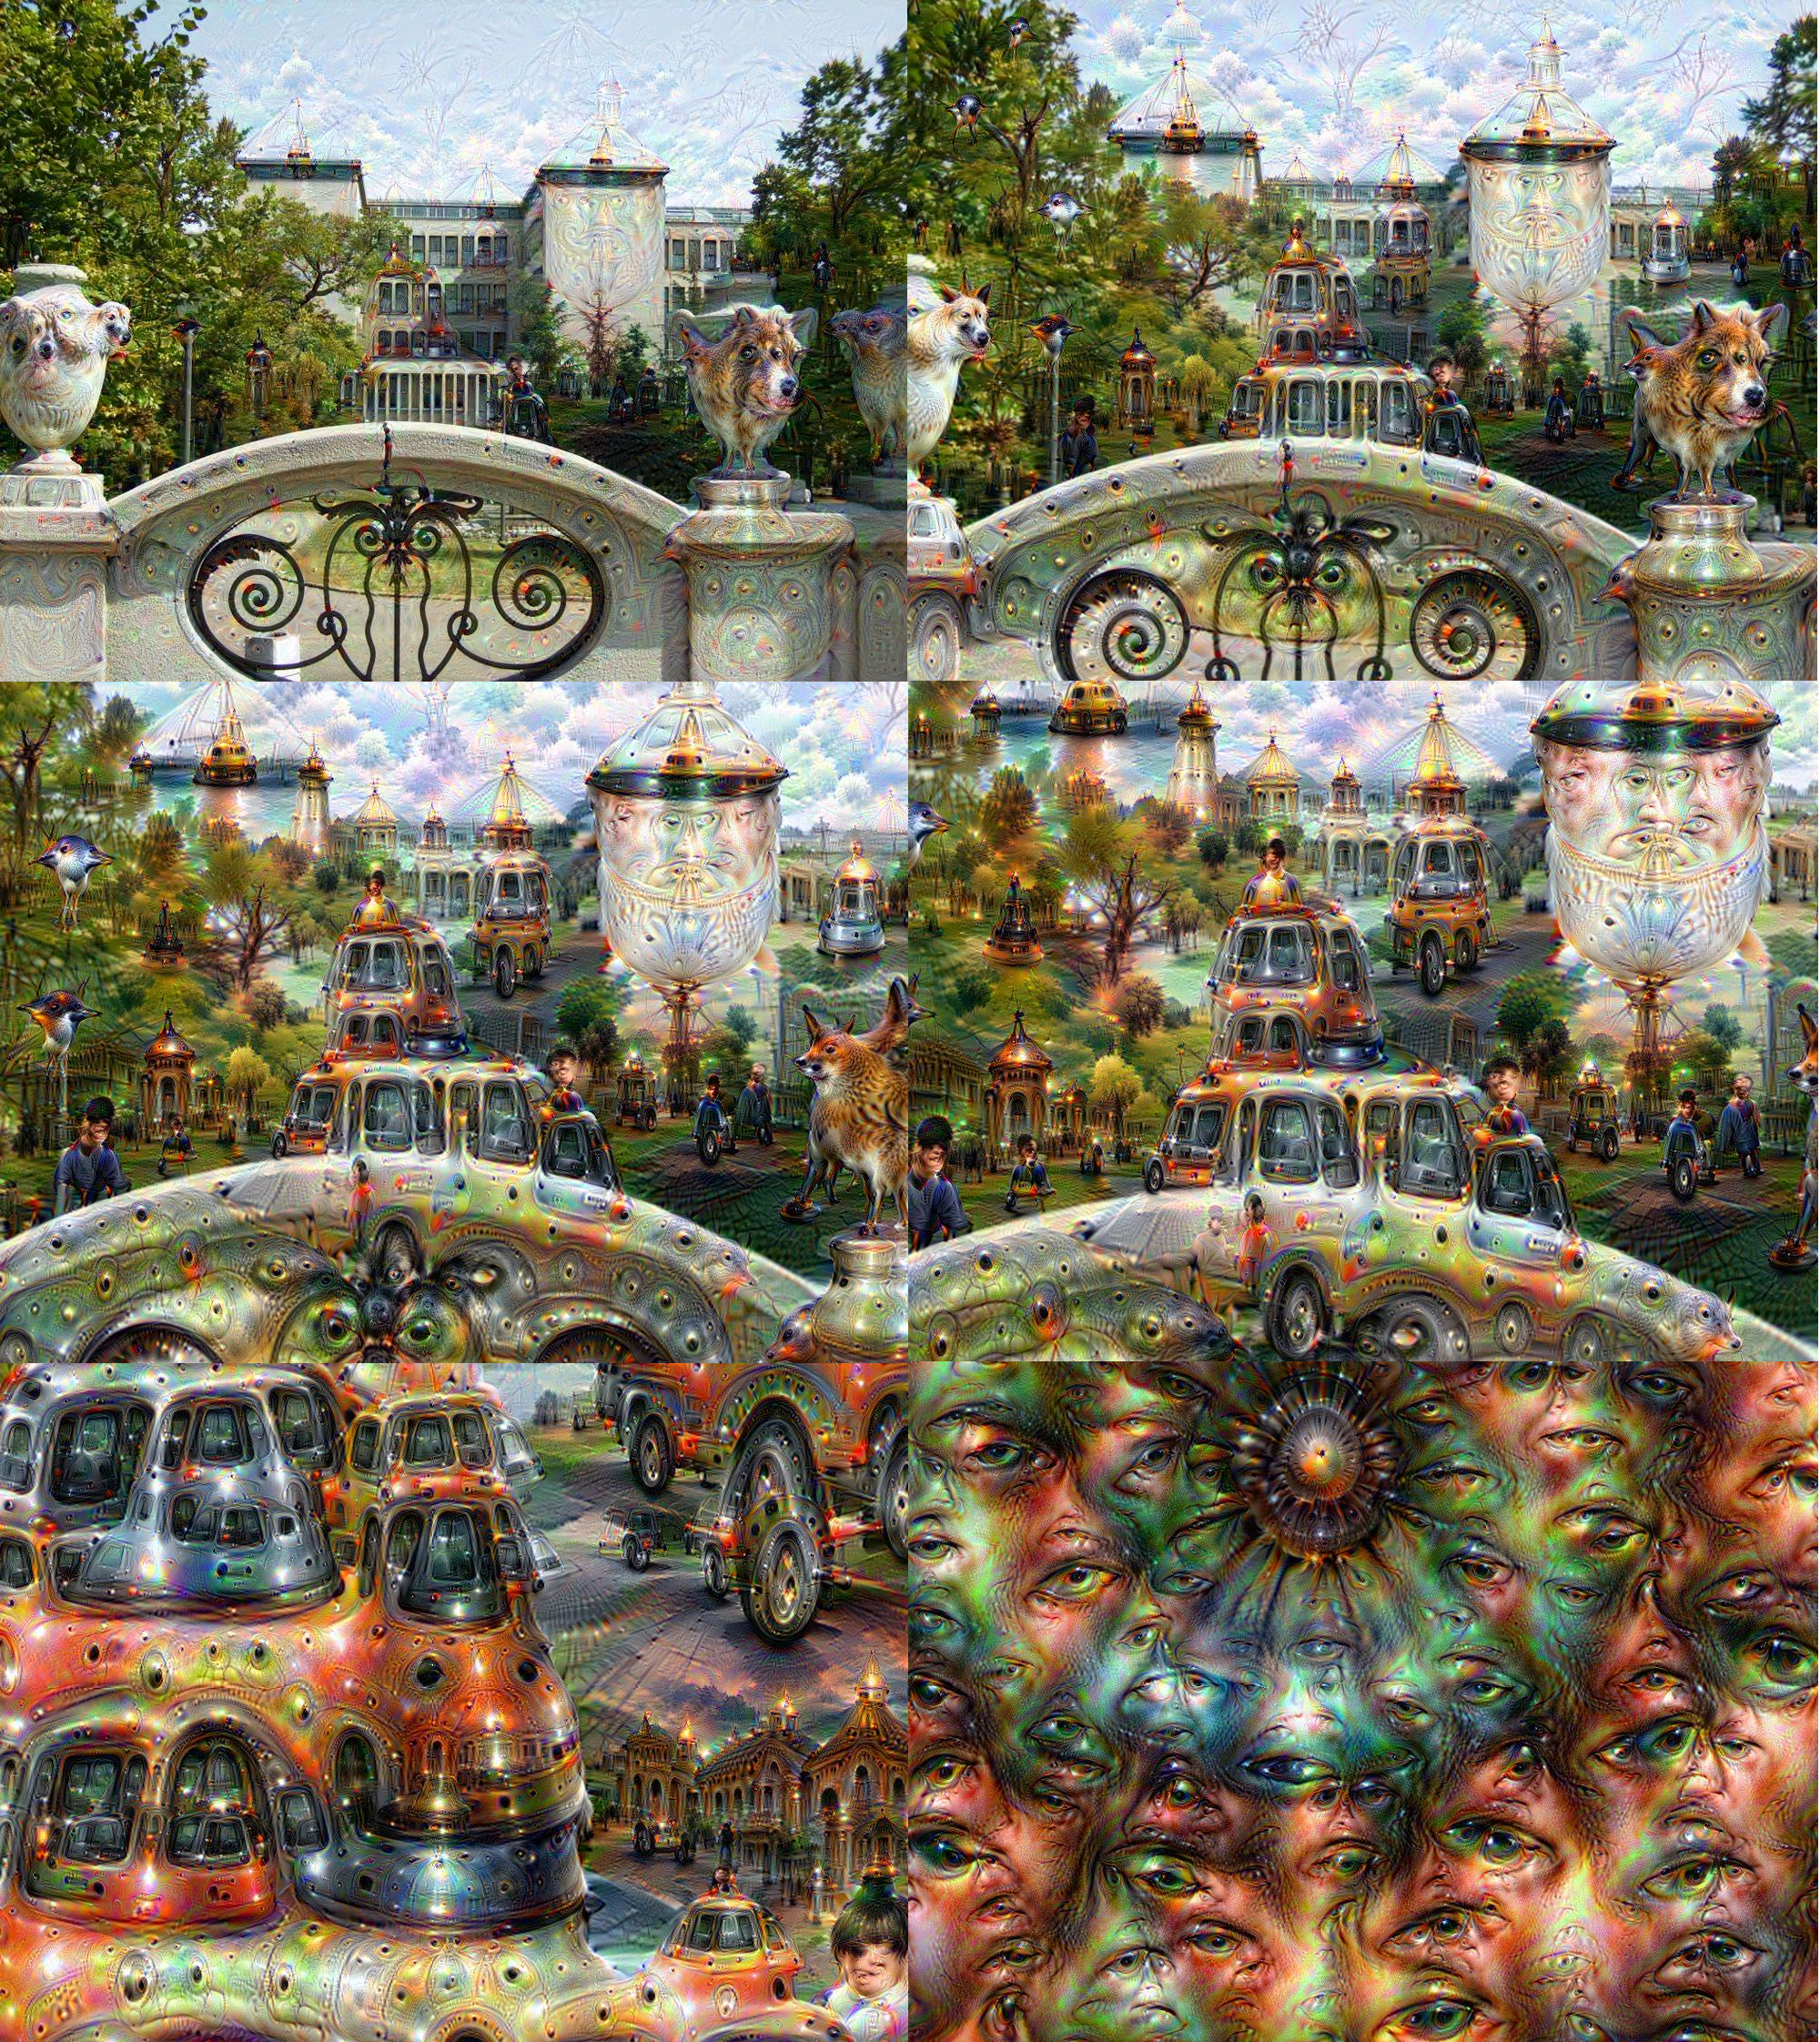
\includegraphics[width=\textwidth]{./resources/matfFun.png}
\end{center}
\caption{Генерисане слике 0, 3, 8, 12, 17, 38, 99 од 100 - крећући се кроз врсте почевши одозго}
\label{fig:matffun}
\end{figure}

Може се користити и слика која наводи генератор. Slika \ref{fig:dreamgenerator} приказује
слику која се користи за навођење, а слика \ref{fig:dreamgeneratedresult} слику која је
добијена.

\begin{minted}[frame=single,framesep=10pt]{python}
# Ucitava se slika koji navodi generisanje
guide = np.float32(PIL.Image.open('flowers.jpg'))
showarray(guide)

end = 'inception_3b/output'
h, w = guide.shape[:2]
src, dst = net.blobs['data'], net.blobs[end]
src.reshape(1,3,h,w)
src.data[0] = preprocess(net, guide)
net.forward(end=end)
guide_features = dst.data[0].copy()

def objective_guide(dst):
    x = dst.data[0].copy()
    y = guide_features
    ch = x.shape[0]
    x = x.reshape(ch,-1)
    y = y.reshape(ch,-1)
    # Izracunava se matrica skalarnog 
    # proizvoda sa slikom koja navodi generisanje
    A = x.T.dot(y)
    # Bira se vrednost koja je najveca
    dst.diff[0].reshape(ch,-1)[:] = y[:,A.argmax(1)]

# Generise se slika koristeci sliku koja navodi generisanje
_=deepdream(net, img, end=end, objective=objective_guide)
\end{minted}

\begin{figure}[h!]
\begin{center}
    \includegraphics[scale=0.5]{./resources/flowers.jpeg}
\end{center}
\caption{Слика која наводи генератор}
\label{fig:dreamgenerator}
\end{figure}

\begin{figure}[h!]
\begin{center}
    \includegraphics[width=\textwidth]{./resources/matfFlowers.jpeg}
\end{center}
\caption{Добијена слике користећи слику навођења}
\label{fig:dreamgeneratedresult}
\end{figure}

% ---------------------------------------------------------------------------------------------------------------------
\section{Закључак}
% ---------------------------------------------------------------------------------------------------------------------
Пројекат \texttt{DeepDream} који се ослања на раније радове \cite{visualizeCovnet, visualizeCovnet1,
visualizeCovnet3, visualizeCovnet4} указује да је постигнуто одређено разумевање
дубинског рада конволутивних неуронских мрежа. Допринео је даљој популаризацији неуронских мрежа и инспирисао
истраживаче да дубље истраже понашање конволутивних мрежа.

Разумевање рада неуронских мрежа и интепретабилност њихових модела и даље остају
отворена значајна тема у области машинског учења, но свакако су постигнути
значајни успеси у визуелизацији рада мрежа у последњих неколико година.

\newpage
\newpage
\addcontentsline{toc}{section}{Литература}
\appendix
\bibliography{literature}
%\bibliographystyle{plain}
\bibliographystyle{unsrt}


\end{document}
